\documentclass{../konspekt}

\title{Elektryczność i Magnetyzm konspekt}

\begin{document}

\begin{multicols}{2}

  \begin{multicols}{2}

    \section{Trygonometria}

    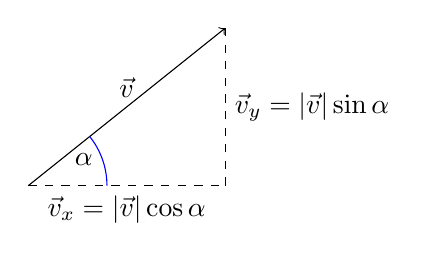
\begin{tikzpicture}
      \coordinate (A) at (0.5,1);
      \coordinate (B) at (3,3);
      \draw [->] (A) -- (B) node [midway, above] {$\vec{v}$};
      \draw [dashed] (A) -- (3,1) node [midway, below] {$\vec{v}_x =
      |\vec{v}| \cos \alpha$};
      \draw [dashed] (3,1) -- (3,3) node [midway, right] {$\vec{v}_y
      = |\vec{v}| \sin \alpha$};
      \draw[draw=blue] (A) ++(0:10mm) arc (0:39:10mm) node[midway,
      left]{$\alpha$};
    \end{tikzpicture}
    \section{Ładunek}

    $$
    q = n \cdot e
    $$
    n - liczba ładunków elementarnych, $e = 1.6 \cdot 10^{-19} C$

  \end{multicols}

  \section{Prawo Coulomba}

  $$
  \vec{F_E} = k \cdot \frac{q_1 \cdot q_2}{r^2} \cdot \vec{r}
  $$
  gdzie $k$ to stała elektrostatyczna($\frac{1}{4\pi\epsilon_0}$,
  $\epsilon_0\approx8.854\cdot10^{-12}\frac{E}{m}$) a $q$ to ładunki.
  $\vec{r}$ to wektor jednostkowy ($|\vec{r}|=1$).
  Dla dipola o ładunkach $q$ i $-q$ w odległości $d$, moment dipolowy
  $p$ jest równy:
  $$
  p = q \cdot d
  $$

  \section{Pole elektryczne}

  $$
  \vec{E}(r) = k \cdot \frac{|q|}{r^2} \cdot \vec{r}
  $$
  Gdzie $r$ to odległość od ładunku, a $q$ to ładunek, tworzący pole
  elektryczne.
  $$
  \vec{F_E} = q \cdot \vec{E}(r)
  $$

  \section{Prawo Gaussa}

  $$
  \frac{Q}{\epsilon_0} = \oint_S E \cdot dS = \frac{1}{\epsilon_0}
  \int_V \rho(r) dr
  $$
  Typowo podczas rozwiązywania zadań, znajdujemy infitisemalnie małą jednostkę
  ciała $dS$ i całkujemy po powierzchni $S$ aby znaleźć całkowite pole
  elektryczne.

  Na skutek nieskończonej linii naładowanej równomiernie
  ładunkiem $\lambda$ mamy:
  $$
  E(r) = \frac{\lambda}{2\pi\epsilon_0 r}
  $$

  Na skutek nieskończonej płaszczyzny naładowanej równomiernie
  ładunkiem $\sigma$ mamy:
  $$
  E = \frac{\sigma}{2\epsilon_0}
  $$

  Na skutek kuli o promieniu $R$ naładowanej równomiernie
  ładunkiem $\sigma$ mamy:
  $$
  E(r) = \frac{\sigma R^2}{\epsilon_0 r^2}
  $$
  \section{Potencjał elektryczny}

  $$
  E = - \nabla V
  $$
  czyli pole elektryczne jest równe gradientowi potencjału
  elektrycznego. $V(r) = k\frac{q}{r}$
  $$
  F_E = qE = -q \nabla V = - \nabla U
  $$
  $U$ to energia potencjalna, a $V$ to potencjał elektryczny.
  $$
  U = qV = k \frac{q_1 q_2}{r}
  $$
  $$
  E_k = \frac{1}{2} m v^2 = qV
  $$

  \section{Kondensatory}

  $$
  C = \frac{Q}{U} = \frac{S \cdot \epsilon_0}{d}
  $$
  gdzie $C$ to pojemność kondensatora, $Q$ to ładunek na
  kondensatorze, a $U$ to napięcie na kondensatorze. Dla kondensatora
  płaskiego $S$ to powierzchnia płytki, a $d$ to odległość między
  nimi. Kondensatory połączone równolegle mają pojemności sumowane:
  $$
  C_{eq} = C_1 + C_2 + \ldots
  $$
  Kondensatory połączone szeregowo mają pojemności odwrotne:
  $$
  \frac{1}{C_{eq}} = \frac{1}{C_1} + \frac{1}{C_2} + \ldots
  $$
  Energia zgromadzona w kondensatorze:
  $$
  W = \int_{0}^{Q} \frac{Q}{C} dQ = \frac{Q^2}{2C} = \frac{1}{2} C V^2
  $$

  \section{Opór elektryczny}

  $$
  I = \frac{Q}{t} = \frac{U}{R} = \frac{P}{U}
  $$
  $R$ to opór elektryczny, $U$ to napięcie, $I$ to natężenie prądu,
  $Q$ to ładunek a $P$ to moc. W kablu o długości $l$ i przekroju $S$,
  opór elektryczny jest równy $R = \rho \frac{l}{S}$, gdzie $\rho$ to
  oporność elektryczna materiału.

  \section{Siła Lorentza}

  $$
  F = q \cdot (E + v \times B)
  $$
  gdzie $F$ to siła Lorentza, $q$ to ładunek, $E$ to pole elektryczne,
  $v$ to prędkość ładunku, a $B$ to pole magnetyczne.

  $$
  F = q \cdot v \cdot B \cdot \sin(\alpha) = q \cdot v \cdot B =
  IlB \cdot \sin(\alpha)
  $$
  gdzie $I$ to prąd w przewodniku,
  a $\alpha$ to kąt między wektorem prędkości a polem magnetycznym.
  Ostatni wzór dotyczy przewodnika o długości $l$ w polu magnetycznym.

  \section{Pole magnetyczne}

  $
  B = \frac{\mu_0 I}{2 R}
  $
  w środku kołowej pętli o promieniu $R$ z prądem $I$.
  $
  B(R) = \frac{\mu_0 I}{2\pi R}
  $
  dla nieskończonej linii naładowanej równomiernie ładunkiem $I$.
  $$
  \oint_{C} B \cdot dl = \mu_0 I
  $$

  \section{SEM}

  $$
  \mathcal{E} = -N \frac{d \Phi}{dt} = Blv
  $$
  SEM to siła elektromagnetyczna, $N$ to liczba zwojów, a $\Phi$
  to strumień magnetyczny.
  $$
  \Phi = BS \cos(\alpha)
  $$

  \section{Zasada prawej ręki}

  \begin{center}
    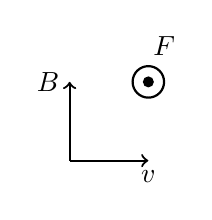
\begin{tikzpicture}
      \draw[thick,->] (0,0) -- (1,0) node[anchor=north] {$v$};
      \draw[thick,->] (0,0) -- (0,1) node[anchor=east] {$B$};

      \draw[thick] (1,1) circle (0.2) node[anchor=south,
      xshift=0.2cm, yshift=0.2cm] {$F$};
      \fill (1,1) circle (0.07);
    \end{tikzpicture}
    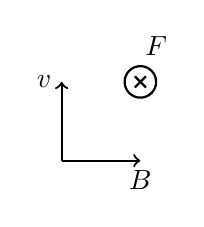
\begin{tikzpicture}
      \draw[thick,->] (0,0) -- (1,0) node[anchor=north] {$B$};
      \draw[thick,->] (0,0) -- (0,1) node[anchor=east] {$v$};

      \draw[thick] (1,1) circle (0.2) node[anchor=south,
      xshift=0.2cm, yshift=0.2cm] {$F$};
      \draw[thick] (0.93,0.93) -- (1.07,1.07);
      \draw[thick] (0.93,1.07) -- (1.07,0.93);
    \end{tikzpicture}
  \end{center}

\end{multicols}

\end{document}
